\documentclass[11pt]{article}
\input{/Users/markwang/.preamble}
\begin{document}
 
\begin{enumerate} 

\item \textbf{Binary Addition with RNN} \\ 
Idea is to have $h_1,h_2,h_3$ activate when the sum of inputs to the hidden layer is at least 1, 2, or 3, respectively. $h_2^{t-1}$ represents the carry over to the sume at step $t$
\[
	\mathbf{U} = 
    \begin{pmatrix}
    1 & 1 \\
    1 & 1 \\
    1 & 1 \\
    \end{pmatrix}
    \quad
    \mathbf{W} = 
    \begin{pmatrix}
    	0 & 1 & 0 \\
        0 & 1 & 0 \\ 
        0 & 1 & 0 \\
    \end{pmatrix}
    \quad 
    \mathbf{b}_h = 
    \begin{pmatrix}
    	-0.5 \\ 
        -1.5 \\ 
        -2.5 \\
    \end{pmatrix}
    \quad 
    \mathbf{v} = 
    \begin{pmatrix}
    	1 \\ -1 \\ 5 \\
    \end{pmatrix}
    \quad 
    h_y = -0.5
\]


\item\textbf{LSTM Gradient}

\begin{enumerate}
\item  
\begin{align*}
    \overline{h^{(t)}} 
    &= \overline{i^{(t+1)}} w_{ih} \sigma(w_{ix}x^{(t+1)} + w_{ih}h^{(t)})(1 - \sigma(w_{ix}x^{(t+1)} + w_{ih}h^{(t)})) \\
    & + \overline{f^{(t+1)}} w_{fh} \sigma(w_{fx}x^{(t+1)} + w_{fh}h^{(t)})(1 - \sigma(w_{fx}x^{(t+1)} + w_{fh}h^{(t)})) \\
    & + \overline{o^{(t+1)}} w_{oh} \sigma(w_{ox}x^{(t+1)} + w_{oh}h^{(t)})(1 - \sigma(w_{ox}x^{(t+1)} + w_{oh}h^{(t)})) \\
    & + \overline{g^{(t+1)}} w_{gh}(1 - \tanh^2 (w_{ox}x^{(t+1)} + w_{oh}h^{(t)})) \\
    \overline{c^{(t)}} &= \overline{c^{(t+1)}} f^{(t+1)} + \overline{h^{(t)}} o^{(t)} (1 - \tanh^2 (c^{(t)})) \\
    \overline{g^{(t)}} &= \overline{c^{(t)}} i^{(t)} \\
    \overline{o^{(t)}} &= \overline{h^{(t)}} \tanh (c^{(t)}) \\
    \overline{f^{(t)}} &= \overline{c^{(t)}} c^{(t-1)} \\
    \overline{i^{(t)}} &= \overline{c^{(t)}} g^{(t)} \\
\end{align*}


\item 
\[
	\overline{w_{ix}} = \sum_{t} \overline{i^{(t)}} x^{(t)} \sigma(w_{ix}x^{(t)} + w_{ih}h^{(t-1)}) (1 - \sigma(w_{ix}x^{(t)} + w_{ih}h^{(t-1)}))
\]
\item In case where forget gate has value very close to 1 and input/output gate close to 0, we have a LSTM block that acts as an identity function
\[
	c^{(t)} \approx c^{(t-1)}
    \qquad 
    \overline{c^{(t)}} \approx 1
\]

\end{enumerate}
\end{enumerate}


\begin{center}
    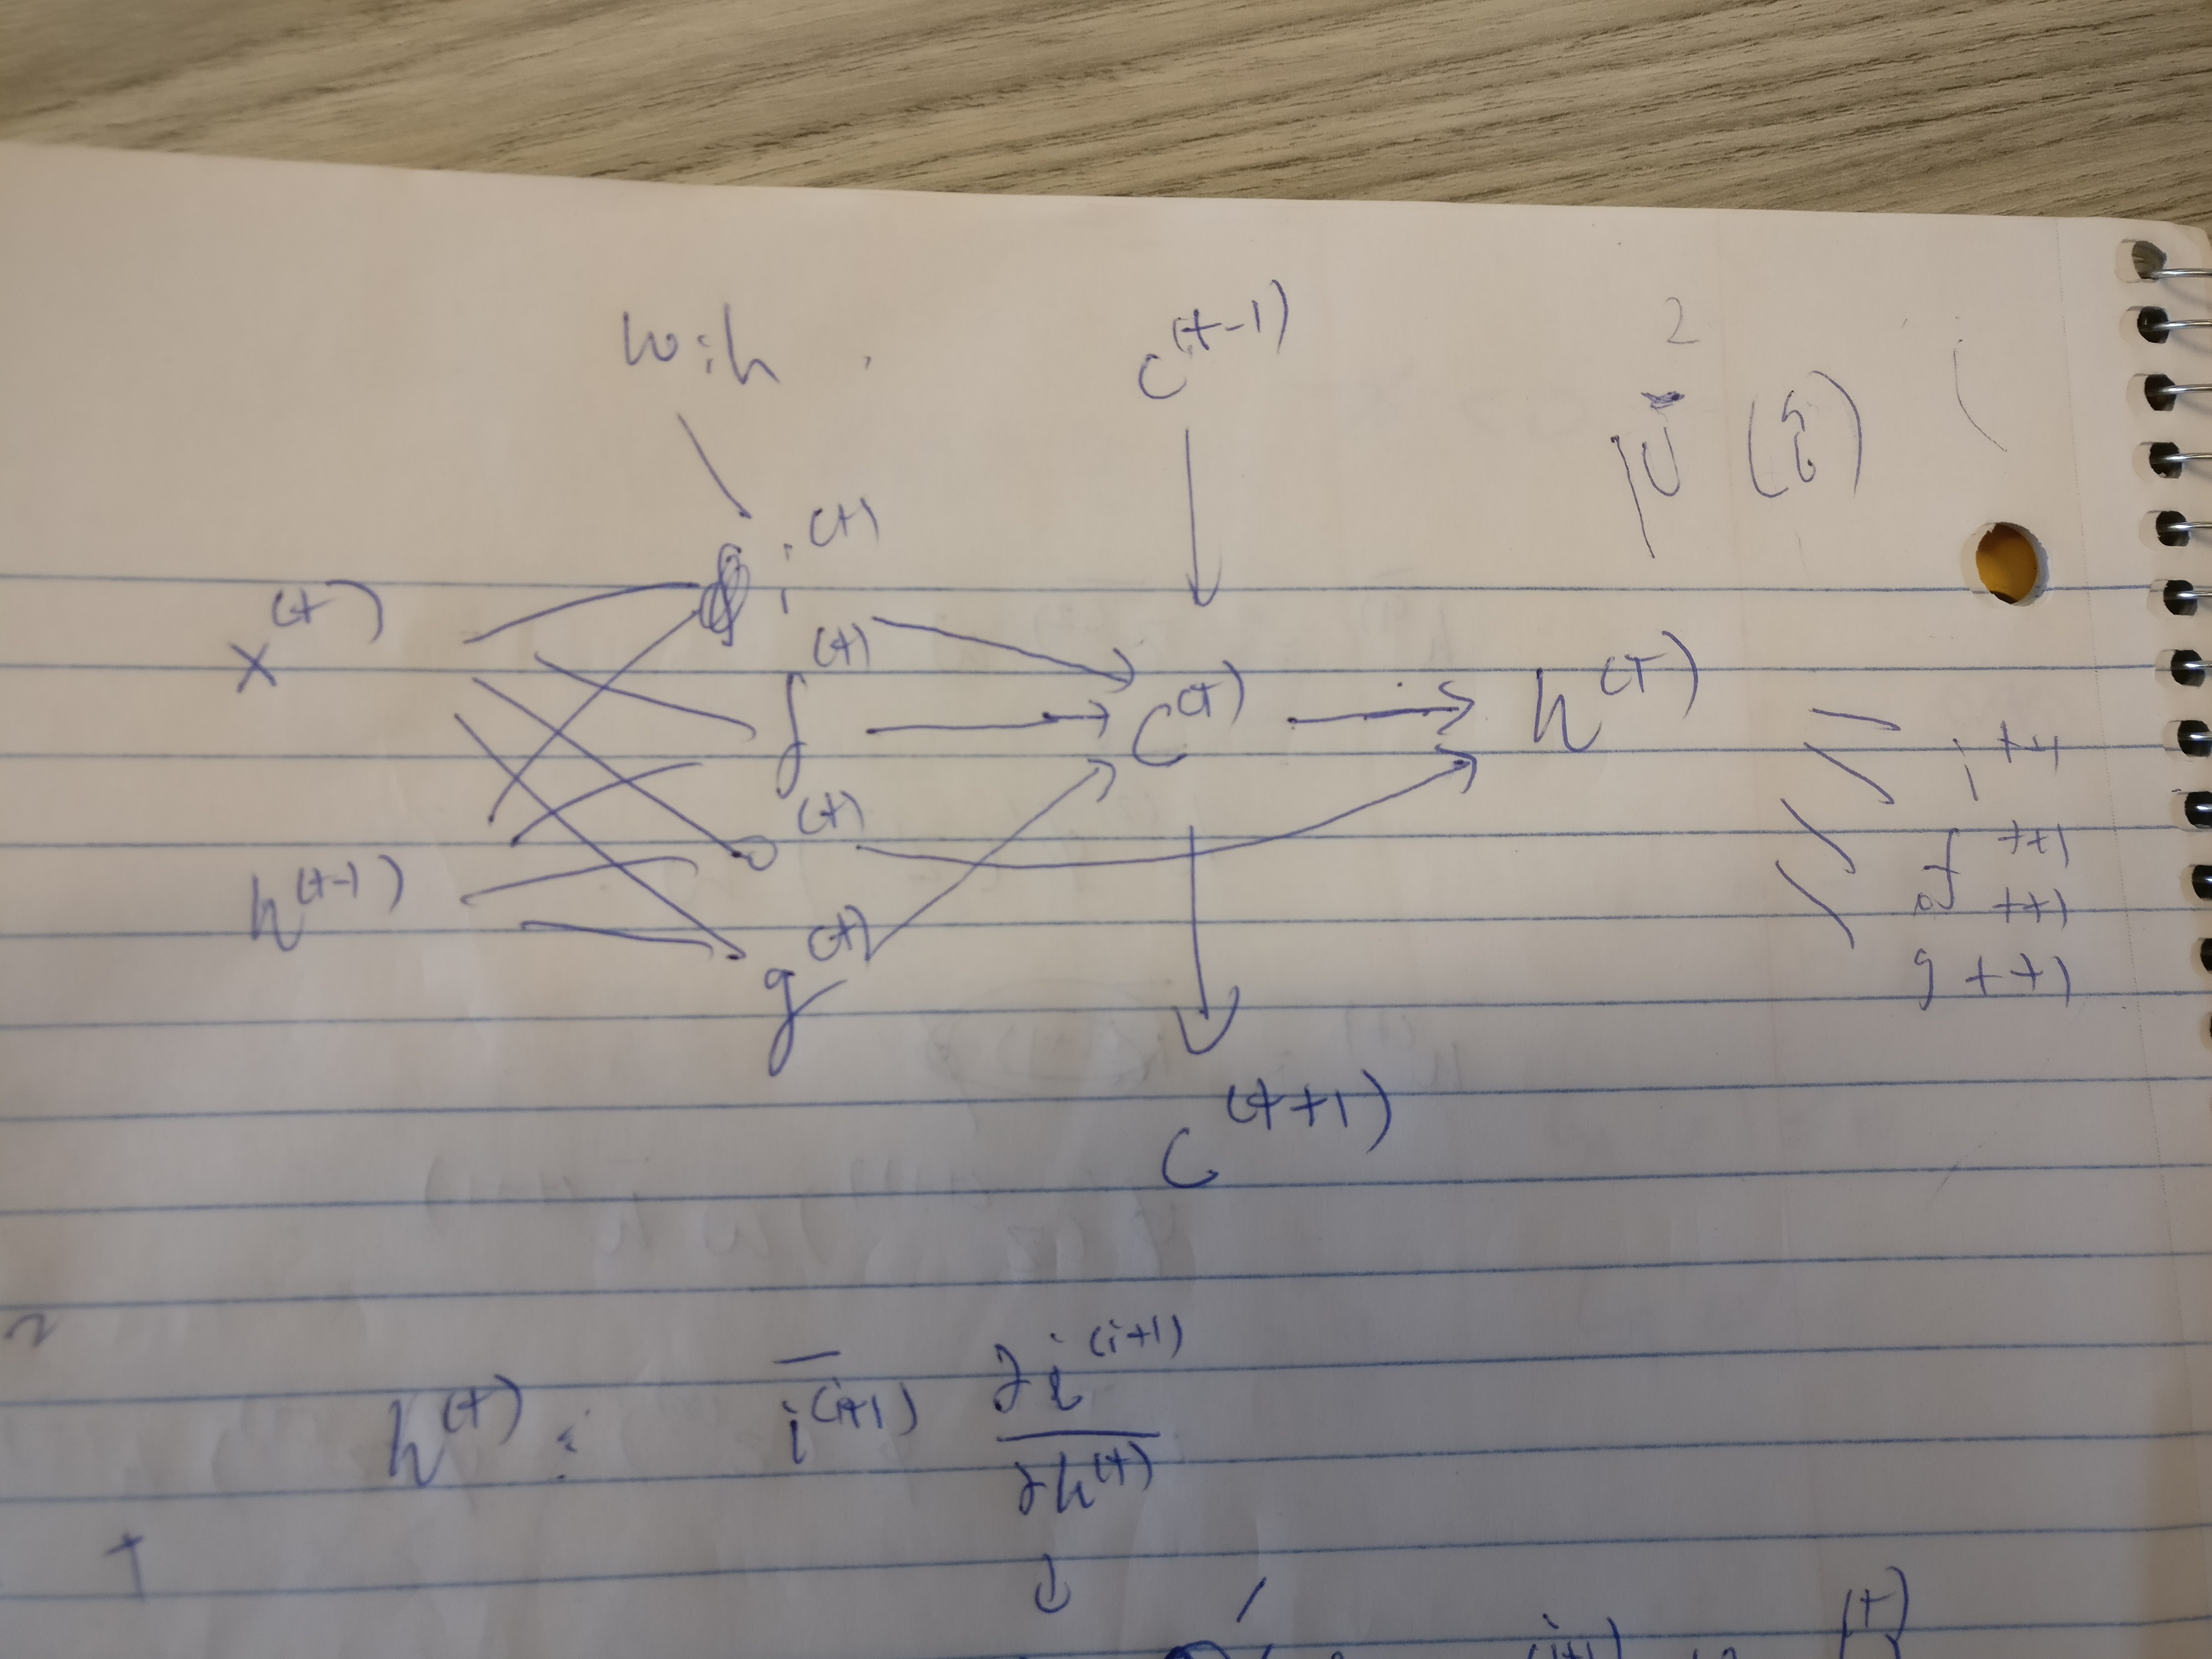
\includegraphics[width=10cm]{computation_graph.jpg}
\end{center}






\end{document}
